%%%%%%%%%%%%%%%%%%%%%%%%%%%%%%%%%%%%%%%%%%%%%%%%%%%%%%%%%%%%%%%%
% MUW Presentation
% LaTeX Template
% Version 1.0 (27/12/2016)
%
% License:
% CC BY-NC-SA 4.0 (http://creativecommons.org/licenses/by-nc-sa/3.0/)
%
% Created by:
% Nicolas Ballarini, CeMSIIS, Medical University of Vienna
% nicoballarini@gmail.com
% http://statistics.msi.meduniwien.ac.at/
%
% Customized for UAH by:
% David F. Barrero, Departamento de Automática, UAH
%%%%%%%%%%%%%%%%%%%%%%%%%%%%%%%%%%%%%%%%%%%%%%%%%%%%%%%%%%%%%%%%%

\documentclass[10pt,compress]{beamer} % Change 10pt to make fonts of a different size
\mode<presentation>

\usepackage[spanish]{babel}
\usepackage{fontspec}
\usepackage{tikz}
\usepackage{etoolbox}
\usepackage{xcolor}
\usepackage{xstring}
\usepackage{multicol}
\usepackage{listings}
\usepackage{tikz}
\usetikzlibrary{matrix,chains,positioning,decorations.pathreplacing,arrows,shapes}

\usetheme{UAH}
\usecolortheme{UAH}
\setbeamertemplate{navigation symbols}{} 
\setbeamertemplate{caption}[numbered]

%%%%%%%%%%%%%%%%%%%%%%%%%%%%%%%%%%%%%%%%%%%%%%%%%%%%%%%%%%%%%%%%%
%% Presentation Info
\title[More Python for Videogames]{More Python for Videogames}
\author{\asignatura\\\carrera}
\institute{}
\date{Departamento de Automática}
%%%%%%%%%%%%%%%%%%%%%%%%%%%%%%%%%%%%%%%%%%%%%%%%%%%%%%%%%%%%%%%%%


%%%%%%%%%%%%%%%%%%%%%%%%%%%%%%%%%%%%%%%%%%%%%%%%%%%%%%%%%%%%%%%%%
%% Descomentar para habilitar barra de navegación superior
\setNavigation
%%%%%%%%%%%%%%%%%%%%%%%%%%%%%%%%%%%%%%%%%%%%%%%%%%%%%%%%%%%%%%%%%

%%%%%%%%%%%%%%%%%%%%%%%%%%%%%%%%%%%%%%%%%%%%%%%%%%%%%%%%%%%%%%%%%
%% Configuración de logotipos en portada
%% Opacidad de los logotipos
\newcommand{\opacidad}{1}
%% Descomentar para habilitar logotipo en pié de página de portada
%\renewcommand{\logoUno}{Images/isg.png}
%% Descomentar para habilitar logotipo en pié de página de portada
%\renewcommand{\logoDos}{Images/CCLogo.png}
%% Descomentar para habilitar logotipo en pié de página de portada
\renewcommand{\logoTres}{Images/ALogo.png}
%% Descomentar para habilitar logotipo en pié de página de portada
%\renewcommand{\logoCuatro}{Images/ELogo.png}
%%%%%%%%%%%%%%%%%%%%%%%%%%%%%%%%%%%%%%%%%%%%%%%%%%%%%%%%%%%%%%%%%

%%%%%%%%%%%%%%%%%%%%%%%%%%%%%%%%%%%%%%%%%%%%%%%%%%%%%%%%%%%%%%%%%
%% FOOTLINE
%% Comment/Uncomment the following blocks to modify the footline
%% content in the body slides. 


%% Option A: Title and institute
\footlineA
%% Option B: Author and institute
%\footlineB
%% Option C: Title, Author and institute
%\footlineC
%%%%%%%%%%%%%%%%%%%%%%%%%%%%%%%%%%%%%%%%%%%%%%%%%%%%%%%%%%%%%%%%%

\begin{document}

%%%%%%%%%%%%%%%%%%%%%%%%%%%%%%%%%%%%%%%%%%%%%%%%%%%%%%%%%%%%%%%%%
% Use this block for a blue title slide with modified footline
{\titlepageBlue
    \begin{frame}
        \titlepage
    \end{frame}
}

\institute{\asignatura}

\begin{frame}[plain]{}
	\begin{block}{Objectives}
		\begin{enumerate}
		\item Being able to manipulate files in Python.
		\item Understand and apply Python serialization (\textit{pickles} and JSON).
		\item Being able to handle exceptions.
%		\item Introduce decorators
		\end{enumerate}
	\end{block}

	\begin{block}{Bibliography}
		\begin{itemize}
			\item The Python Tutorial. \textit{Section 7.2: Reading and writing files}. \href{https://docs.python.org/3/tutorial/inputoutput.html\#reading-and-writing-files}{(Link)}
			\item The Python Tutorial. \textit{Chapter 8: Errors and Exceptions}. \href{https://docs.python.org/3/tutorial/errors.html}{(Link)}
		\end{itemize}
	\end{block}
\end{frame}

{
\disableNavigation{white}
\begin{frame}[shrink]{Table of Contents}

 	\frametitle{Table of Contents}
  	\begin{multicols}{2}
  		\tableofcontents
    	\end{multicols}

 %\frametitle{Table of Contents}
 %\tableofcontents
  % You might wish to add the option [pausesections]
\end{frame}
}


\section{Reading and writing files}

\subsection{Path}

\begin{frame}[fragile]{Reading and writing files}{Path}
    \begin{block}{Path}
	A string that identifies a file in a file system
    \end{block}

	\begin{columns}
 	  \column{.50\textwidth}
		On \textbf{Linux}, the path is denoted by: \\
\begin{verbatim}
path = '/tmp/prueba.txt'
\end{verbatim}
 	  \column{.50\textwidth}
		On \textbf{Windows}, the path is denoted by: \\
\begin{verbatim}
path = 'C:\Windows\Temp'
\end{verbatim}
		And it is represented  in Python by:\\
\begin{verbatim}
path = 'C:\\Windows\\Temp'
\end{verbatim}
		But by also using \textit{raw string}:
\begin{verbatim}
path = r'C:\Windows\Temp'
\end{verbatim}
	\end{columns}
\end{frame}

\subsection{Opening files}
\begin{frame}[fragile]{Reading and writing files}{Opening files}
	All file operations are made through a \textit{file object}
		\begin{itemize}
		\item \small{First of all: Call the \texttt{open()} function}
		\end{itemize}

	\begin{block}{\texttt{open()}}
	\vspace{-0.2cm}
\begin{verbatim}
open(filename[, mode])
\end{verbatim}
	\vspace{-0.2cm}
	Return: An object file\\
	\vspace{-0.2cm}
	\begin{itemize}
	\item \textit{filename}: Path
	\item \textit{mode}: Characters describing how the file will be used
		\begin{itemize}
		\item \textit{r}: Read mode, \textit{w}: Write mode (overwrites file)% lectura por defecto. W: borra el contenido anterior, r+: lectura y escritura; a: append
        \item \textit{r+}: r/w mode, no truncation; \textit{w+}: r/w mode, truncation
        \item \textit{a}: Write, appending mode
		\item \textit{b}: Binary mode, text mode by default
		\end{itemize}
	\end{itemize}
	\end{block}

	\smallskip

	\begin{alertblock}{}
	Always, always, always close the file: \texttt{f.close()} (unless in a \texttt{with} clause)
	\end{alertblock}
\end{frame}

\subsection{Reading files}
\begin{frame}[fragile]{Reading files (I)}
	\begin{block}{The \texttt{read()} function}
	\vspace{-0.2cm}
\begin{verbatim}
f.read([size])
\end{verbatim}

	\vspace{-0.2cm}
	Return: the specified number of bytes
	\begin{itemize}
	\item \textit{size}: The number of bytes to be read from the file. Default reads the whole file
	\end{itemize}
	\end{block}
\textbf{Option 1}: Read the entire file (\texttt{f.read()})
\begin{verbatim}
>>> f = open("/tmp/file", 'r')
>>> f.read()
'This is the entire file.\\n'
>>> f.read()
''
>>> f.close()
\end{verbatim}
	
\end{frame}

\begin{frame}[fragile]{Reading files (II)}
	\textbf{Option 2}: Read a single line (\texttt{f.readline()})
\begin{verbatim}
>>> f = open("/tmp/file2", 'r')
>>> f.readline()
'This is the first line of the file.\n'
>>> f.readline()
'This is the second line of the file\n'
>>> f.readline()
''
>>> f.close()
\end{verbatim}

\end{frame}

\begin{frame}[fragile]{Reading files (III)}
	\textbf{Option 3}: Read lines as list (\texttt{f.readlines()})
\begin{verbatim}
>>> f = open("/tmp/file2", 'r')
>>> f.readlines()
['This is the first line of the file.\n',
'This is the second line of the file\n']
>>> f.close()
\end{verbatim}

	\textbf{Option 4}: Read in a loop
\begin{verbatim}
f = open("/tmp/file2", 'r')
for line in f:
    print(line, end='')
f.close()
\end{verbatim}
\end{frame}

\begin{frame}[fragile]{Example}{}
	\begin{exampleblock}{Calculating the average of characters per line of file \texttt{example.txt}}
	\vspace{-0.2cm}
	\lstinputlisting[numbers=left]{code/char_average_line.py}
	\vspace{-0.2cm}
	\end{exampleblock}
\end{frame}

\subsection{Writing files}

\begin{frame}[fragile]{Writing files (I)}
	\begin{block}{The \texttt{write()} function}
	\vspace{-0.2cm}
\begin{verbatim}
f.write(string)
\end{verbatim}

	\vspace{-0.2cm}
	Return: Number of written bytes
	\begin{itemize}
	\item \textit{string}: String to write
	\end{itemize}
	\end{block}

	\textbf{Example 1}: Write a line
	 % si el archivo se crea con modo w+: se sobrescribe lo que hubiera al estar ya creado.
	 % no se lee luego nada porque el puntero está posicionado al final y no hay más.
	\begin{verbatim}
>>> f = open("/tmp/file", 'w+')
>>> f.write('This is a test\n')
15
>>> f.read()
'' 
>>> f.close()
\end{verbatim}

\end{frame}

\begin{frame}[fragile]{Writing files (II)}
	

	\textbf{Example 2}: Write a number % se tiene que pasar a string el número
\begin{verbatim}
>>> f = open("/tmp/file", 'w+')
>>> f.write(str(42))
2
>>> f.close()
\end{verbatim}
\end{frame}

\subsection{Useful methods}
\begin{frame}[fragile]{Useful methods}

	\begin{tabular}{c|l}\hline
  	\sc Method & \sc Description  \\\hline
  	\texttt{f.tell()} & Returns the pointer's position \\
  	\texttt{f.seek(n)} & Moves the pointer \texttt{n} bytes \\
  	\texttt{f.close()} & Closes a file. Use it always! \\\hline
  	\end{tabular}

\begin{verbatim}
>>> f = open("/tmp/file", 'rb+')
>>> f.write(b'0123456789abcdef')
16
>>> f.seek(5)
5
>>> f.read(1)
b'5'
>>> f.close()
\end{verbatim}
\end{frame}
% que hagan: obtener el número de bytes de un archivo, el archivo es muy, muy largo: léalo no completo sino en fragmentos de 64 bytes, leer de línea en línea (lo más frecuente), 
% o todas las líneas de una vez, bucles sobre, directamente, las líneas del archivo. Escribir usando write y writelines (porporcionar finales de línea adecuadamente). Copia de un archivo (del todo o por líneas), de 1024 en 1024, 

% CADENA UNICODE!
\subsection{With}

\begin{frame}[fragile]{\texttt{With} (I)}
	\begin{columns}
	\column{.6\textwidth}
	\begin{block}{The \texttt{with} clause}
	\vspace{-0.2cm}
\begin{verbatim}
with open(path, mode) as file:
    ...
\end{verbatim}
	\end{block}

	\column{.4\textwidth}

	It simplifies file operations
	\begin{itemize}
	\item No need to close files
    \item Better exception handling
	\end{itemize}
    \end{columns}

    
	\begin{columns}
	\column{.45\textwidth}
	\begin{exampleblock}{}
	\begin{verbatim}
f = open('file')
print(f.read())
f.close()
\end{verbatim}
    \end{exampleblock}

	\column{.05\textwidth}
    $\Rightarrow$

	\column{.50\textwidth}
	\begin{exampleblock}{}
	\begin{verbatim}
with open('file') as file:
    print(file.read())
\end{verbatim}
    \end{exampleblock}

    \end{columns}
\end{frame}

\begin{frame}[fragile]{With (II)}
	\begin{exampleblock}{Hello, world}
	\vspace{-0.2cm}
	\lstinputlisting[numbers=left]{code/hello-with.py}
	\vspace{-0.2cm}
	\end{exampleblock}
\end{frame}

\begin{frame}[fragile]{With (III)}
	\begin{exampleblock}{Reading a line each time}
	\vspace{-0.2cm}
	\lstinputlisting[numbers=left]{code/cierreautomatico.py}
	\vspace{-0.2cm}
	\end{exampleblock}

	\begin{columns}
	\column{.40\textwidth}
    \centering $\Uparrow$
	\begin{exampleblock}{names.txt}
	\lstinputlisting[basicstyle=\scriptsize, numbers=left]{code/nombres.txt}
	\end{exampleblock}
	\column{.50\textwidth}
    \centering $\Downarrow$
	\begin{exampleblock}{Output}
	\lstinputlisting[basicstyle=\scriptsize]{code/output.txt}
	\end{exampleblock}
	\end{columns}
	
\end{frame}

\section{Serialization}

\begin{frame}[fragile]{Serialization}{Introduction}
    What happens if we need to store complex data structures?
		\begin{itemize}
			\item Think about lists, dictionaries or even objects ...
		\end{itemize}
    What happens if we need to transmit complex data structures?

	\begin{columns}
	\column{.6\textwidth}
	\begin{block}{Serialization}
    Converting a data object into a sequence of bytes
	\end{block}
    \end{columns}

    \bigskip

    We can easily store and even transmit sequences of bytes ...
	\begin{itemize}
        \item ... and also reconstruct our original data
	\end{itemize}
	There are several serialization technologies: Pickles, JSON, XML, ...

\end{frame}

\subsection{The pickle module}

\begin{frame}[fragile]{Serialization}{The \texttt{pickle} module}
	Given an object \texttt{x} and a file object \texttt{f} ...
\begin{verbatim}
>>> pickle.dump(x, f) 
>>> x = pickle.load(f)
\end{verbatim}
\end{frame}
% byte of p. 93 -- cPickle más rápido

\begin{frame}[plain]{Serialization}{The \texttt{pickle} module: Examples}
	\begin{exampleblock}{Save a list  to a file}
	\vspace{-0.2cm}
	\lstinputlisting[numbers=left]{code/pickle_example_list_dump.py}
	\vspace{-0.2cm}
	\end{exampleblock}

	\begin{exampleblock}{Load a list from a file}
	\vspace{-0.2cm}
	\lstinputlisting[numbers=left]{code/pickle_example_list_load.py}
	\vspace{-0.2cm}
	\end{exampleblock}
\end{frame}

\subsection{The JSON module}

\begin{frame}[fragile]{Serialization}{The \texttt{JSON} module: Introduction}
	\begin{columns}
 	  \column{.40\textwidth}
		JSON: \textit{JavaScript Object Notation}
		\begin{itemize}
		\item Data format for hierarchical data
        	\item Created in 2001 for stateless client-server communication
	        \item Text-based
		\item Interoperable (pickles only for Python)
	        \item Complex data structures
		\end{itemize}

 	  \column{.60\textwidth}
        \begin{exampleblock}{filename.json}
		\begin{lstlisting}[basicstyle=\scriptsize]
{
  "firstName": "John",
  "isAlive": true,
  "age": 27,
  "address": {
    "streetAddress": "21 2nd Street",
    "city": "New York",
    "state": "NY",
  },
  "phoneNumbers": [ "111", "333" ]
}
\end{lstlisting}
        \end{exampleblock}
	\end{columns}
\end{frame}

\begin{frame}[fragile]{Serialization}{The \texttt{JSON} module: Examples}
	\begin{exampleblock}{Save a list to a file}
	\vspace{-0.2cm}
	\lstinputlisting[numbers=left]{code/json_example_list_dump.py}
	\vspace{-0.2cm}
	\end{exampleblock}

	\begin{exampleblock}{Load a list from a file}
	\vspace{-0.2cm}
	\lstinputlisting[numbers=left]{code/json_example_list_load.py}
	\vspace{-0.2cm}
	\end{exampleblock}
\end{frame}

\section{Exceptions}
\subsection{Motivation}

\begin{frame}[fragile]{Exceptions}{Motivation}
	Errors happen
	\begin{itemize}
		\item We need a mechanism to handle errors
	    \item Some errors happen before execution (\textit{syntax errors})

\begin{verbatim}
>>> while True print('Hello world')
  File "<stdin>", line 1
    while True print('Hello world')
                   ^
  SyntaxError: invalid syntax
\end{verbatim}

		\item Others are only detected in execution (\textit{runtime errors})

\begin{verbatim}
>>> int("hola")
Traceback (most recent call last):
  File "<stdin>", line 1, in <module>
ValueError: invalid literal for int() with base 10: 'hola'
\end{verbatim}

    \end{itemize}
    $\Rightarrow$We need tools to handle errors: \alert{Exceptions}
\end{frame}

\subsection{Definition}

\begin{frame}[fragile]{Exceptions}{Exception definition (I)}
	\alert{Exception}: An error that disrupts the normal execution flow
	\begin{itemize}
		\item File not found, division by zero, invalid argument, etc
		\item Code cannot be executed
		\item Elegant solution to handle errors
	\end{itemize}
\end{frame}

\begin{frame}{Exceptions}{Exception definition (II)}
    \begin{columns}
 	   \column{.50\textwidth}
		\centering Call stack
		\centering 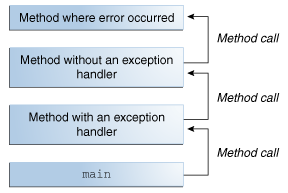
\includegraphics[width=0.8\linewidth]{figs/exceptions-callstack.png}

  	\column{.50\textwidth}
		\textit{Call stack}: Sequence of invoked methods
	\end{columns}
\end{frame}

\begin{frame}{Exceptions}{Exception definition (III)}
    \begin{columns}
 	   \column{.60\textwidth}
		\centering Exception handling
		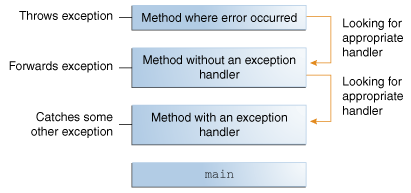
\includegraphics[width=0.8\linewidth]{figs/exceptions-errorOccurs.png}

  	\column{.60\textwidth}
		When an error happens ...
		\begin{enumerate}
		\item Code execution is stopped
		\item An exception is thrown
		\item The interpreter goes back in the call stack
		\item When the interpreter finds an exception handler, it is executed
		\end{enumerate}
		The exception handler catches the exception, the program finishes otherwise
	\end{columns}
\end{frame}

\begin{frame}{Exceptions}{Exception definition (IV)}
	\lstinputlisting{code/stack.txt}
\end{frame}

\subsection{Handling exceptions}
\begin{frame}{Exceptions}{Handling exceptions (I)}
	Handling an exception requires a try-except statement
	\begin{itemize}
		\item \texttt{try}: Encloses the vulnerable code
		\item \texttt{except}: Code that handles the exception (\textit{catch} in Java/C++)
	\end{itemize}

    \begin{columns}
 	   \column{.60\textwidth}
	\begin{block}{try-except statement}
	\vspace{-0.2cm}
		\lstinputlisting{code/try.py}
	\vspace{-0.2cm}
	\end{block}
	\end{columns}
\end{frame}

\begin{frame}{Exceptions}{Handling exceptions (II)}
    \begin{columns}
 	   \column{.90\textwidth}
	\begin{exampleblock}{try-except example}
	\vspace{-0.2cm}
		\lstinputlisting[numbers=left]{code/try-example.py}
	\vspace{-0.2cm}
	\end{exampleblock}
	\end{columns}
	\bigskip
	The exception type contains the error
\end{frame}

\begin{frame}{Exceptions}{Handling exceptions (III)}
	\vspace{-0.2cm}
    \begin{columns}
 	   \column{.90\textwidth}
	\begin{exampleblock}{try-except example}
	\vspace{-0.2cm}
		\lstinputlisting[numbers=left]{code/try-example2.py}
	\vspace{-0.2cm}
	\end{exampleblock}
	\end{columns}
	\bigskip
	New Python elements
		\begin{itemize}
		\item Raise
        \item Exception as object
		\end{itemize}
\end{frame}

\subsection{Clean-up actions}
\begin{frame}{Exceptions}{Clean-up actions}
	\vspace{-0.2cm}
	Sometimes we need to execute code under all circumstances
	\begin{itemize}
		\item Typically clean-up actions: Close files, database connections, sockets, etc
		\item The \textbf{finally} clause solves this problem
	\end{itemize}

	\vspace{-0.2cm}
    \begin{columns}
 	   \column{.60\textwidth}
	\begin{exampleblock}{Example}
	\vspace{-0.2cm}
		\lstinputlisting[numbers=left]{code/try-finally.py}
	\vspace{-0.2cm}
	\end{exampleblock}

	\end{columns}
\end{frame}

%\section{Decorators}
%\begin{frame}{Decorators}

%	TODO
%	\vspace{-0.2cm}
%	Sometimes we need to execute code under all circumstances
%	\begin{itemize}
%		\item Typically clean-up actions: Close files, database connections, sockets, etc
%		\item The \textbf{finally} clause solves this problem
%	\end{itemize}

%	\vspace{-0.2cm}
%    \begin{columns}
% 	   \column{.60\textwidth}
%	\begin{exampleblock}{Example}
%	\vspace{-0.2cm}
%		\lstinputlisting[numbers=left]{code/try-finally.py}
%	\vspace{-0.2cm}
%	\end{exampleblock}

%	\end{columns}
%\end{frame}

\end{document}
